\section{Arquitecturas Propuestas}

\subsection{Arquitectura Híbrida TN-NTN}

Aunque los enfoques convencionales tratan las redes terrestres y no terrestres como dominios separados, la verdadera convergencia 6G exige una arquitectura unificada desde el diseño. 

Partiendo de arquitecturas de referencia para adaptividad en sistemas satelitales \cite{Basciani2026_RA} y de propuestas recientes de conectividad integrada \cite{Ullah2026_D2D}, presentamos una arquitectura híbrida TN-NTN con tres planos claramente definidos: acceso, control y orquestación. El plano de acceso soporta enlaces directos D2D tanto a estaciones base terrestres como a satélites LEO, habilitando roaming seamless sin intervención explícita del usuario. 

La estructura modular permite que un dispositivo estándar 6G perciba y seleccione dinámicamente el mejor enlace según condiciones de canal, calidad de servicio y políticas de red. Esta aproximación preserva compatibilidad con estándares 3GPP mientras introduce flexibilidad cognitiva que los diseños actuales tienden a subaprovechar.

\subsection{Payloads Regenerativos y Orquestación}

Resulta revelador observar cómo la transición desde payloads bent-pipe hacia procesadores regenerativos cambia radicalmente las posibilidades de integración TN-NTN. 

En la arquitectura propuesta, los satélites LEO incorporan payloads con capacidades de demodulación/decodificación y re-encapsulación a bordo, lo que reduce significativamente la latencia ida-vuelta y permite optimizaciones locales de recursos. Inspirados en arquitecturas candidatas para servicios conjuntos de comunicación y posicionamiento \cite{DeGaudenzi2026_NTN}, incluimos un módulo de orquestación distribuida que coordina recursos entre gateways terrestres, constelaciones LEO y core network 6G.

Esta orquestación inteligente utiliza gemelos digitales de red para predecir movilidad y asignar recursos de forma proactiva, mitigando en gran medida los efectos del handover frecuente en órbitas bajas.

\subsection{Soporte D2D en Bandas Sub-7 GHz y Ka}

Uno de los desafíos persistentes al habilitar D2D satelital radica en reconciliar las restricciones de los dispositivos comerciales con las demandas del canal espacial. 

Nuestro marco define soporte dual para bandas sub-7 GHz (principalmente n256 y n1) y banda Ka para enlaces de mayor capacidad. El modelo de link budget D2D-NTN propuesto se expresa como:

\begin{equation}
P_{rx} = P_{tx} + G_{tx} + G_{rx} - L_{path} - L_{atm} - L_{Doppler} + \Delta_{margin}
\label{eq:link_budget}
\end{equation}

donde se incorporan términos específicos de compensación Doppler y desvanecimiento causado por el movimiento relativo.

\begin{figure}[t]
\centering
% 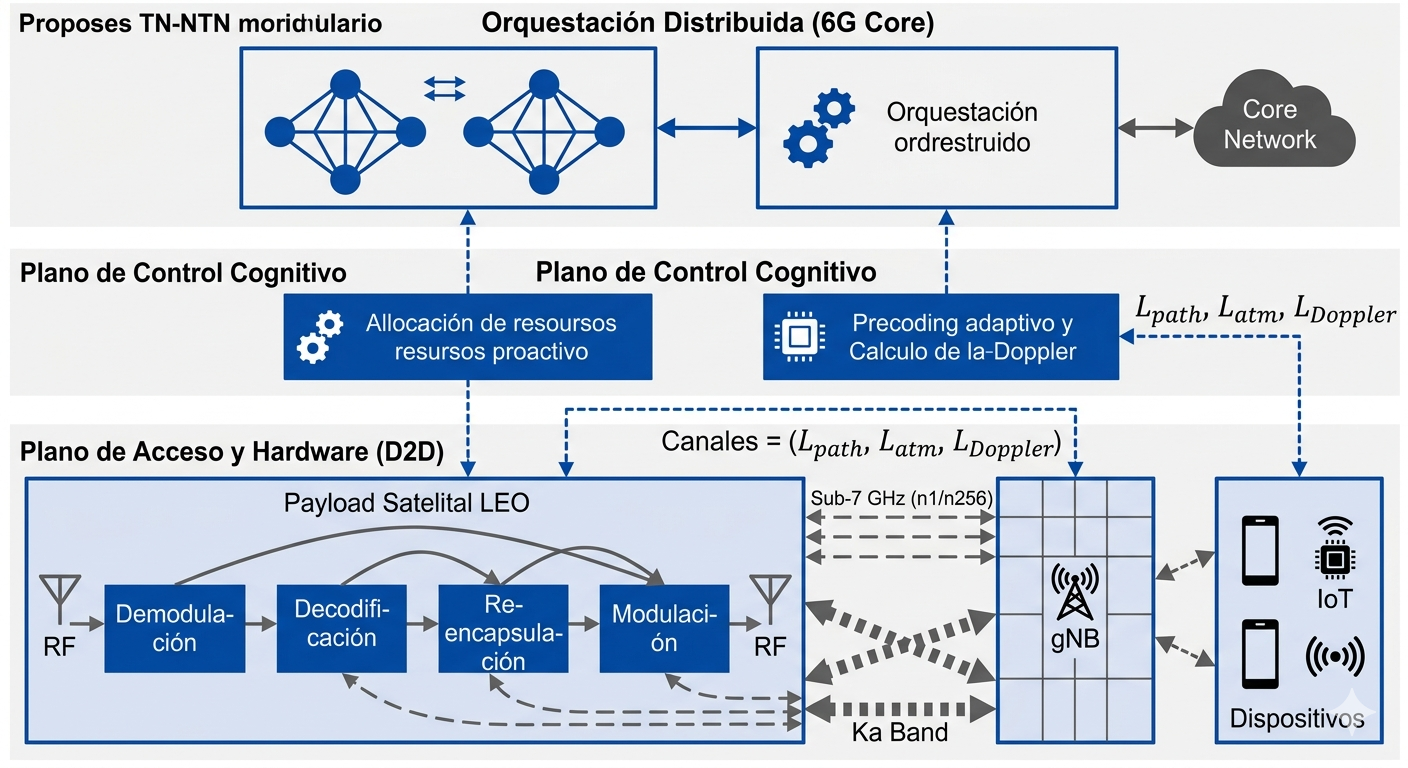
\includegraphics[width=0.95\linewidth]{fig3.png}
\includegraphics[width=0.95\linewidth]{codes/fig3.drawio.pdf}
\caption{Diagrama del marco propuesto de arquitectura híbrida TN-NTN con soporte D2D nativo para ecosistema 6G.}
\label{fig:proposed_architecture}
\end{figure}

La integración de técnicas de precodificación, beamforming dinámico y control de potencia adaptativo permite mantener enlaces D2D estables incluso bajo condiciones adversas. Aunque esta flexibilidad multi-banda incrementa la complejidad del terminal, ofrece un equilibrio práctico entre cobertura global y rendimiento.

En conjunto, la arquitectura propuesta establece un equilibrio viable entre madurez tecnológica y ambición 6G, proporcionando una base sólida para implementaciones futuras.